\chapter{The sPHENIX detector}
The sPHENIX detector is part of the Relativistic Heavy Ion Collider (RHIC) complex at Brookhaven National Laboratories (BNL) in Upton, New York. 
RHIC is one of two major circular particle colliders in the world, the other of which is the Large Hadron Collider at CERN in Geneva, Switzerland. 
Over the course of the sPHENIX experiment which will run from run 23 until RHIC ceases operations after run 25, RHIC will be colliding gold nuclei and protons with run 23 having been dedicated to commissioning Au+Au running, 
run 24 dedicated to p+p with three weeks of Au+Au for further tracking commissioning and run 25 dedicated to physics running in Au+Au collisions. 
RHIC runs with a center of mass energy of $\sqrt{s} = 200 GeV$ for both protons and gold, and additionally is the sole collider that collides polarized protons, which allows for more in depth studies of spin physics. 
At RHIC, sPHENIX's forerunner, the Pioneering High Energy Nuclear Interaction eXperiment (PHENIX), performed the first measurement of the Quark Gluon Plasma droplets \cite{QGP_droplets} in nuclei-nuclei collisions. 

sPHENIX is designed to offer significant upgrades to PHENIX, specifically providing increased coverage with hadronic and electromagnetic calorimeters, increasing effectiveness in studies of jets and heavy flavor at mid-to-high Bjorken x \cite{sPHENIX_TDR}\cite{sPHENIX_whitepaper}\cite{sPHENIX_physics_goals}
Broadly, sPHENIX can be broken into three categories of subsystem: Calorimeters, Tracking and Event characterization.

sPHENIX is constructed around a 1.5 Tesla superconducting magnet, cooled by liquid helium, which was previously used on the BABAR experiment at SLAC, with the outer hadronic calorimeter sitting on the outer radius of the magnet, as see in fig \ref{fig:sphenix_detector}
\begin{figure}
	\includegraphics[width=0.9\textwidth]{sphenix_detector}
	\caption{The sPHENIX detector. The Zero Degree Calorimeter is not pictured but is located further along the beam pipe.}
	\label{fig:sphenix_detector}
\end{figure}
\section{Calorimetry}
	\subsection{Analog Digital Converters and Data Acquisition}
		Beyond the purposes and hardware of the detector itself, one can further characterize the subsystems of sPHENIX into streaming readout and non-streaming detectors, broadly distinguishing the tracking detectors from other subsystems. 
		The non-streaming detectors all use a common data acquisition pipeline and data format. 
		These detectors are readout to analog digital converters boards with 64 channels each, which are then grouped into sets of 3 called an "XMIT" group, which is then read to the data format as a "packet" of 192 channels. 
		Each packet is transmitted from the detector to the computing center on a separate fiber optic cable that is then read into a digitizer which forms groups of (at most) eight packets that are then assigned to individual data acquisition servers. 
		The digitizing process allows for readback into the detector through a global trigger and timing module, where each DAQ server, can issue commands and readback to an event building logic that will then flow back to the detector controlling the same XMIT groups. 
		Each set of (at most) 4 XMIT groups is arranged into a crate with a single crate controller that receives trigger and timing information distributed via a global timing and level 1 trigger module (GL1/GTM) that is then processed through a clockmaster for each digitizer rack, which will hold between 1 and 4 crates, depending of the needs of the subsystem. 
		The data read out to each DAQ server is then stored in the "Purschke Raw Data Format" or prdf file that provides an event structure consisting of a header with some identifying information and separate headers for each packet, but is otherwise comprehensible as an ASCII file. 
		This event structure allows for easy offline combination of events across the calorimeters while keeping individual file size buffers relatively small, as each packet has timing information along with an event number relative to the run that is inherited form the timing module. 
		This DAQ configuration is currently used for the calorimeters, the event plane detector and the minimum bias detector, which allows for faster event building to verify data quality and alignment. 
		The tracking detectors utilize a streaming readout format that creates event pools that are then associated with beam crossing timings provided by the RHIC clock and can be matched onto the GTM timing in offline analysis. 
		This process is slow, and the fully implementation of event combination is still under development, not accounting for event reconstructions which involves track matching across subsystems and will be discussed in section \ref{sec:events}.
		\subsubsection{ADC Zero Suppression}
			\label{sec:zero_supr}
			While this system allows for a simplified readout of the calorimetry system, one expects that, for the average event, most of the towers will be dominated by noise, thus one wastes significant computational resources on reading and storing data that will be immediately discarded.
			This decreases readout rates, runs the risk of filling the storage systems and increases the likelihood of register errors that require restarting runs; in summary, these null data points give no useful physics and hurt our ability to consistently take data. 
			The ADC and readout electronic systems are thus equipped with a zero suppression system that allows for onboard discrimination and data reduction. 
			At the FPGA level, each channel is individually evaluated by taking a post-pre measurement and comparing to a threshold derived from studies of average noise in each channel
			\begin{equation}
				ADC_{\textrm{sample 6}} - ADC_{\textrm{sample 0}} > E_{\textrm{cut off}}
				\label{eq:post_pre}
			\end{equation}
			Where the evaluation shown in eq (\ref{eq:post_pre}) assumes that the ADC readout has been properly timed in relative to the trigger such that the peak of well formed data should be centered near sample 6 (of 12, 16 or 31), and one can take a cutoff with resolution as wide as a single number and as granular as a tower-by-tower volume. 
			Studies have been performed at sPHENIX to establish good thresholds for this zero-suppression approach and validate that this will not introduce biasing into the detector \cite{Lis2020}. 
			%put in an averaging noise plot here 
	\subsection{Hadronic Calorimeters}
		sPHENIX's power in jet physics comes in large part from its calorimeter systems, including two separate hadronic calorimeters. 
		The outer and inner hadronic calorimeter (OHCal and IHCal respectively) are both divided into 24 bins in $\eta$ with coverage of $|\eta| \leq 1.1$  and full $\varphi$ coverage with 64 bins in $\varphi$, grouped into 32 sectors across $\eta$ in each calorimeter. 
		Each hadronic calorimeter therefore has tower size of $\delta \eta = 0.092$ and $\delta \varphi=0.098$.  
		The outer hadronic calorimeter is constructed of steel and sits outside of the magnet, with inner radius of $r=1.82$ m and outer radius of $r=2.69$ m. 
		The inner hadronic calorimeter is constructed of aluminum and sits just inside the magnet, with inner radius of $r=1/16$ m and outer radius of $r=1.37$ m. 
		Each tower corresponds to a readout board that sums readout from four scintillator paddles in the inner HCAL and five scintillator paddles in the outer HCAL embedded into the calorimeter as show in fig. \ref{fig:hcal}. 
		These interface boards form a single readout channel, and can be individually tested via a pulser system that injects charge into the interface board testing readback independent of scintillator response, and LED system that injects a fixed pulse of light into the scintilators to test behavior of the Silicon Photomultipliers (SiPMs). 
		Output of each of these systems is shown in fig \ref{fig:hcal_tests}
		\begin{figure}
			%need to figure out how to do the subfigures for this 
			\begin{subfigure}[t]{0.4\textwidth}
				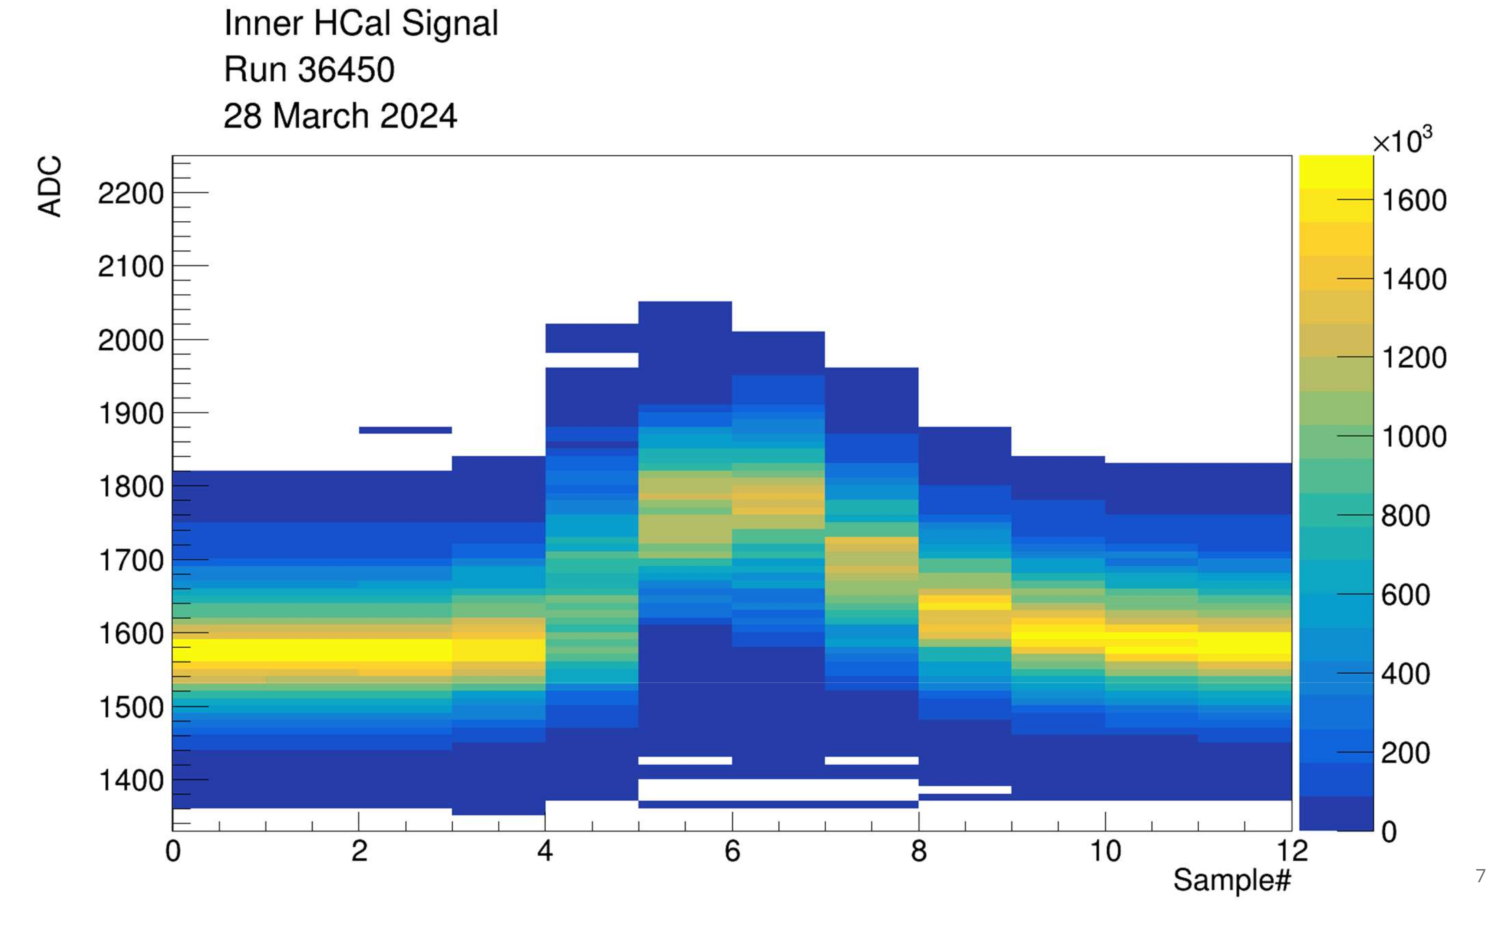
\includegraphics[width=0.9\textwidth]{pulser_waveform}
				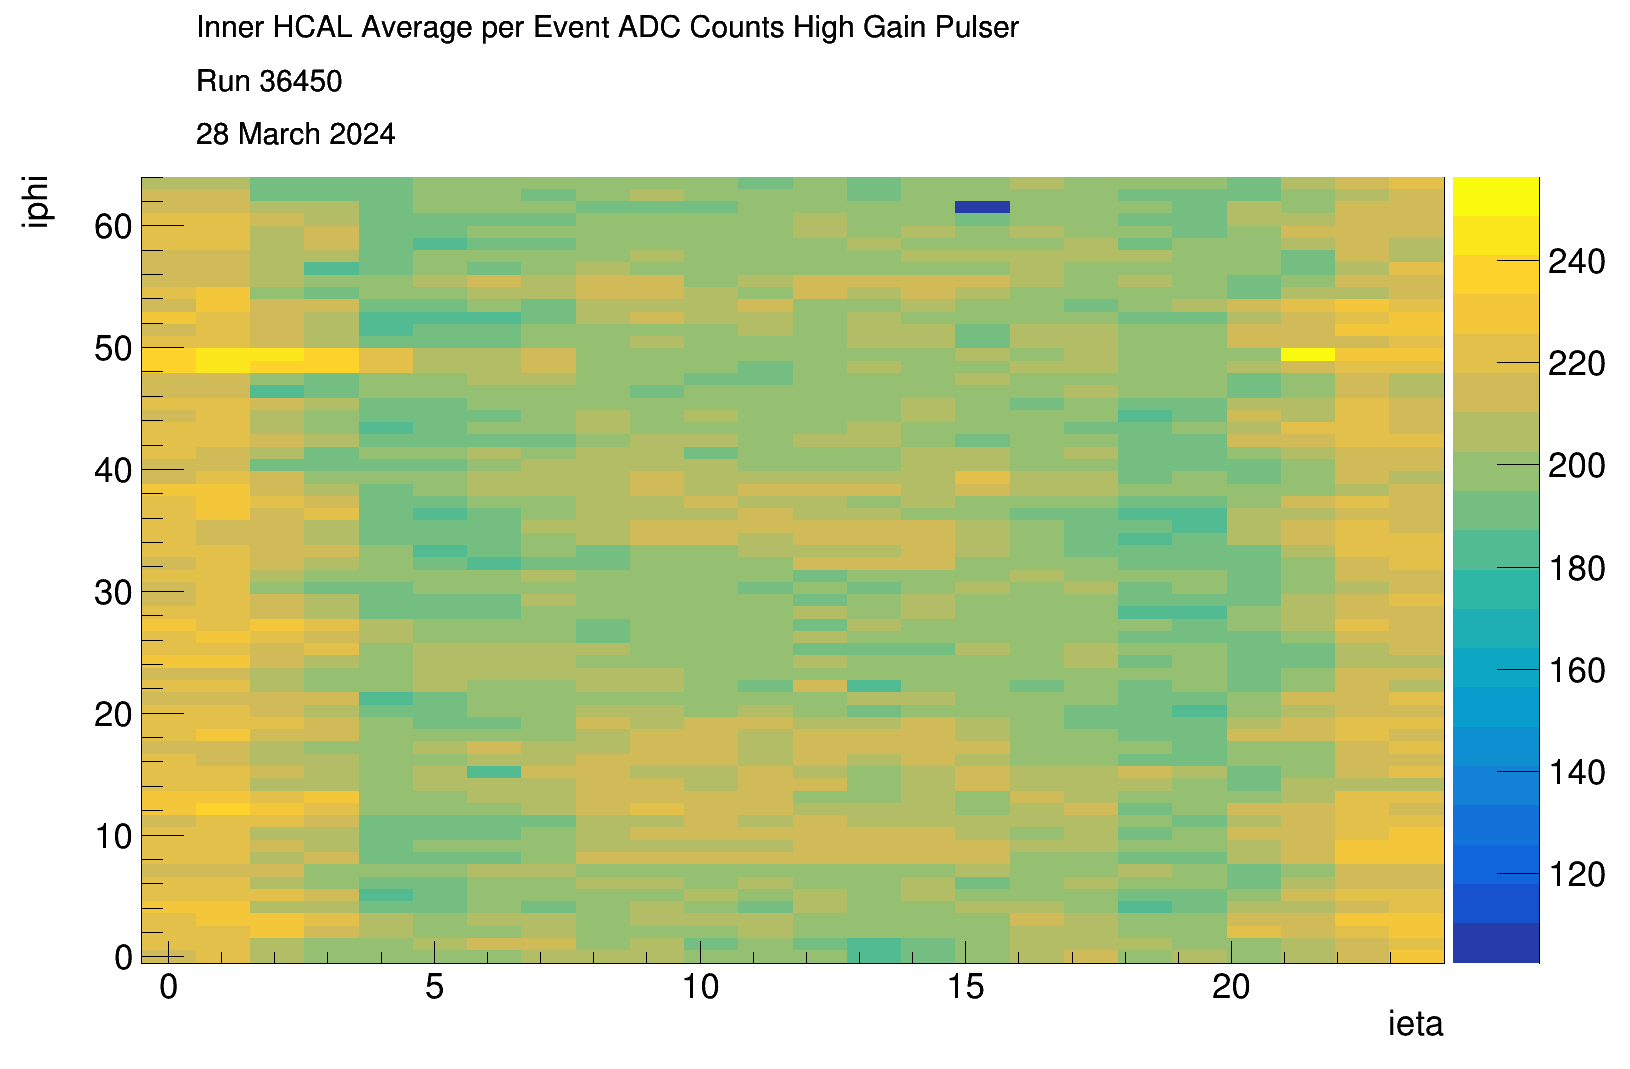
\includegraphics[width=0.9\textwidth]{ihcal_pulser.png}
				\caption{Charge Injection Pulse. This system allows for direct testing of electronics without detector response}
			\end{subfigure}
			\hfill
			\begin{subfigure}[t]{0.4\textwidth}
				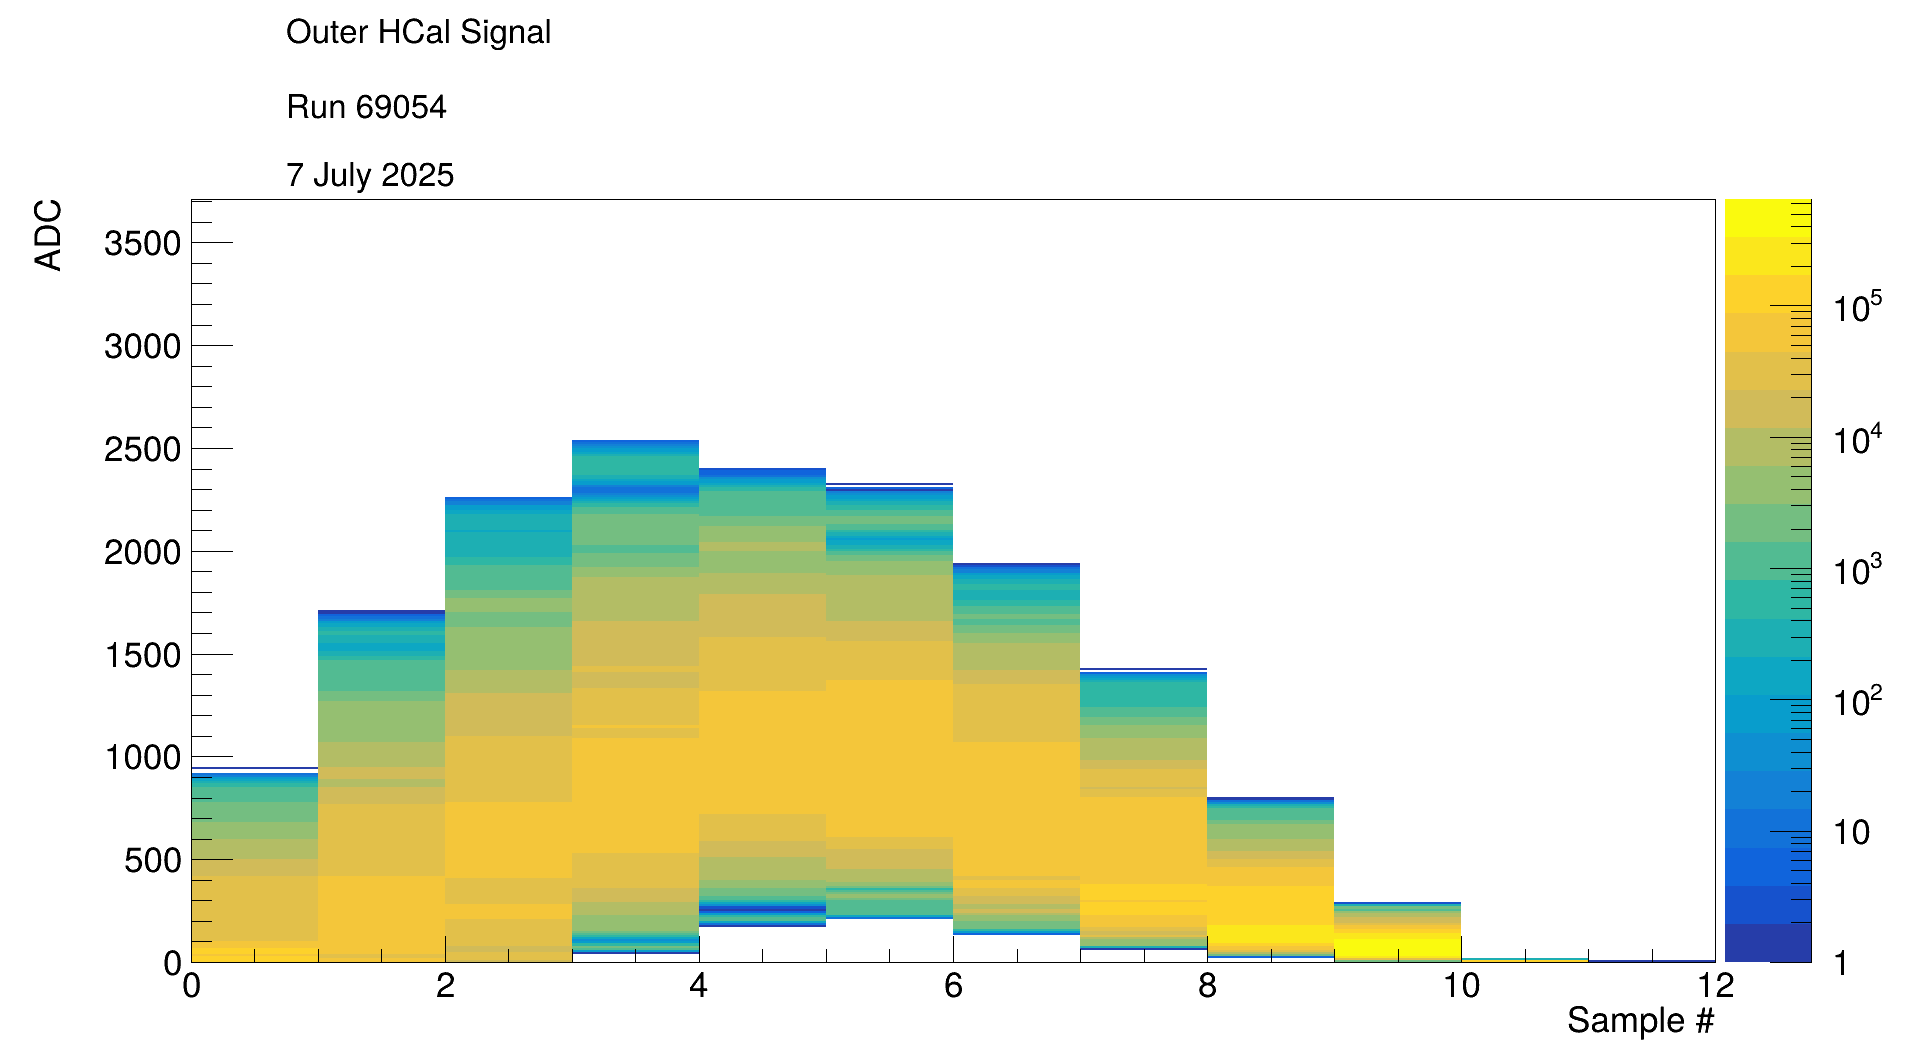
\includegraphics[width=0.9\textwidth]{ohcal_led_signal.png}
				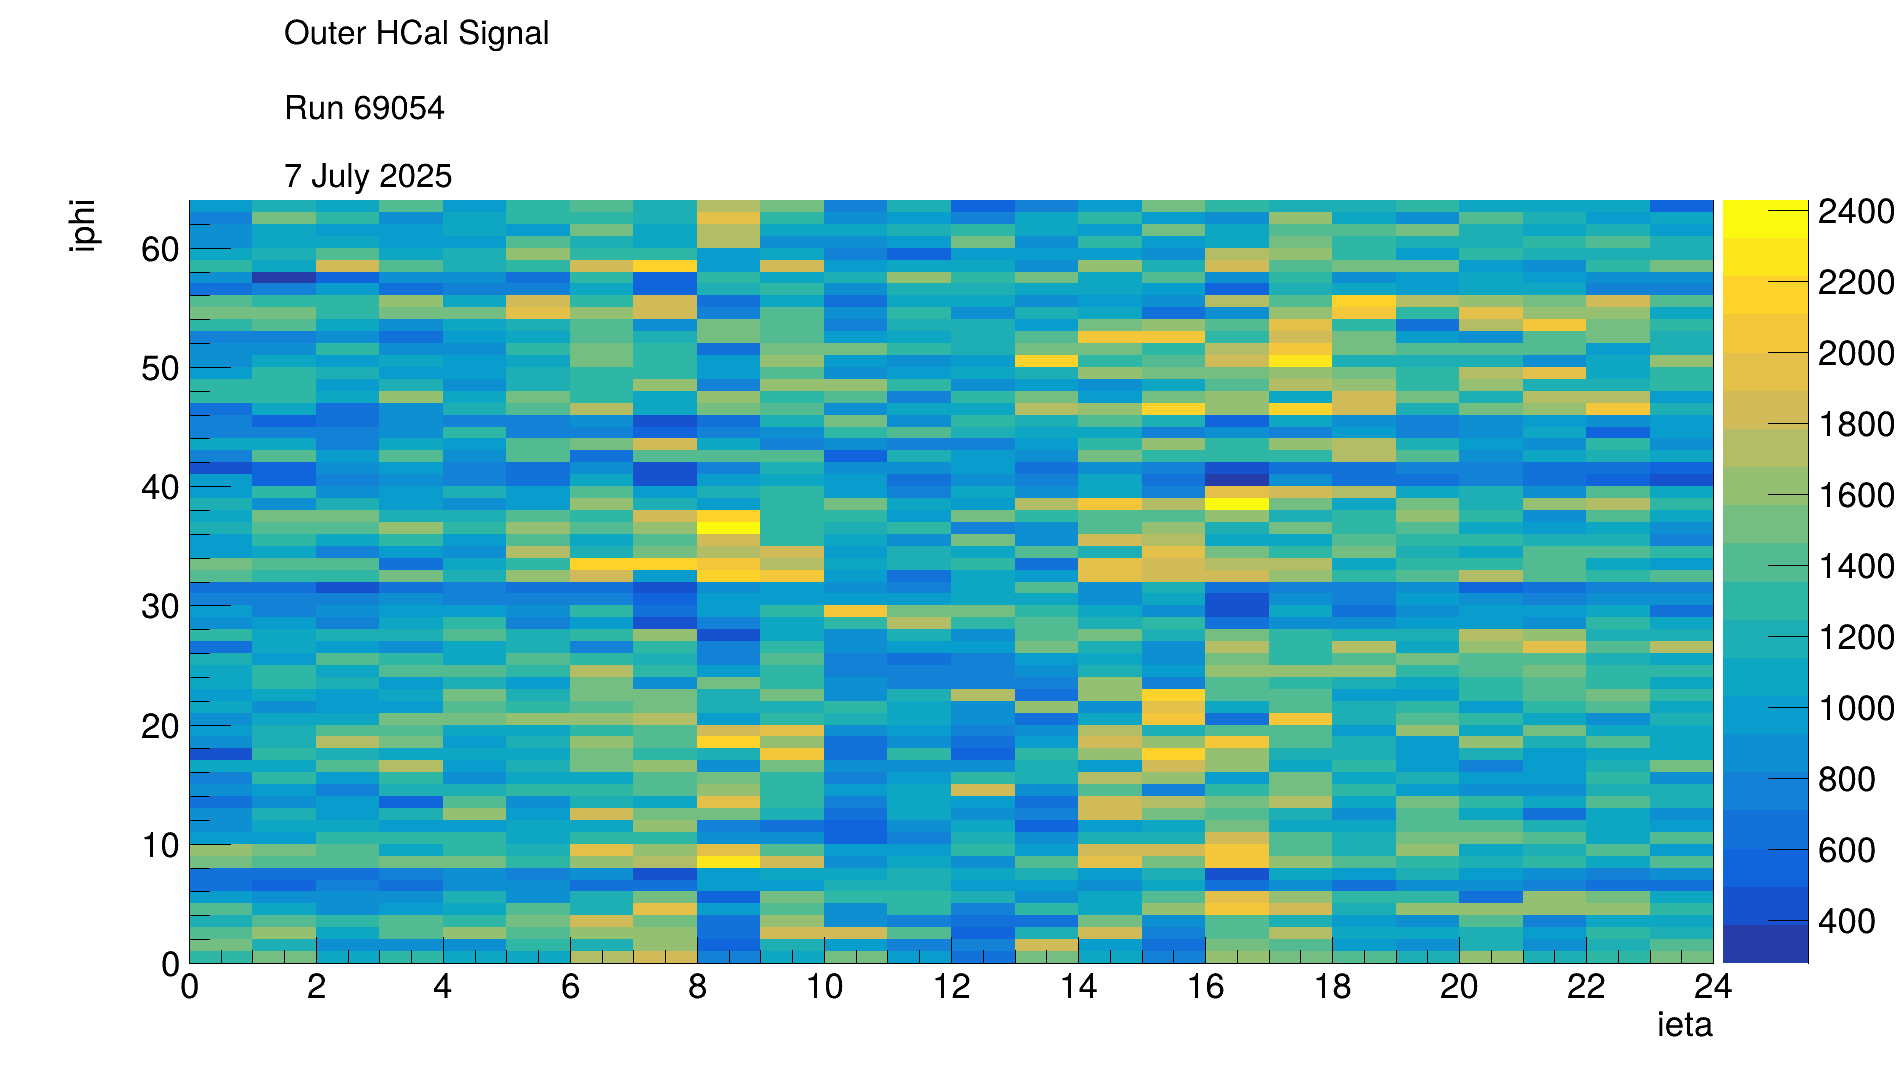
\includegraphics[width=0.9\textwidth]{ohcal_led_energy.png}
				\caption{LED pulse. This allows for testing of the full readback system and light response}
			\end{subfigure}
				\caption{Top: Persistence Waveform. Bottom: Energy distribution averaged across $10^{5}$ events}
			\label{fig:hcal_tests}
		\end{figure}
		\subsubsection{Calibration}
			The hadronic calorimeters were initially calibrated through use of cosmic ray muons, matching the spectra to Monte Carlo 
			generated through EcoMug and GEANT4 \cite{HCal_Calib}. 
			This calibration is updated throughout the run via continued cosmic ray studies in between physics data taking, in addition
			to ongoing work on in-situo calibrations using tower-slope methods \cite{tower_slope_hcal}. 
			These calibrations have yielded an average conversion factor for the OHCal of and the IHCal of %*put ing the factor here*%
	\subsection{Electromagnetic Calorimeter}
		Moving in one layer from the hadronic calorimeter, the Electromagnetic Calorimeter (EMCal) has the same coverage in $\eta-\varphi$ space,
		but has 16 times as many towers with 96 bins in $\eta$ and 256 bins in $\varphi$. 
		The EMCal is constructed of blocks of tungsten with embedded scintillating fibers, 
		and has inner radius $r=0.9$ m and outer radius of $r=1.16$ m.
		Similarly to the HCals, the EMCal is also equipped with a pulser and LED, although the increased number of towers and higher variability 
		in response requires that different pulse widths be used for separate sets of towers to prevent saturation and clipping on the LED pulse.
		\subsubsection{Calibration}
			The EMCal was calibrated to the $\pi^0$ mass through the $\pi^0 \rightarrow \gamma \gamma$ decay channel with additional corrections
			applied via the tower slope. 
			The mean $m_{\pi^0}$ and width are used as quality assurance plots to monitor radiation damage to the EMCal on an ongoing basis and provide updated calibrations throughout the runs.

	\subsection{Zero Degree Calorimeter}
		The Zero Degree Calorimeter (ZDC) is a small transverse energy hadron detector that positioned outside of the experiment hall, in the tunnels along the beam pipe, 18 m from the interaction point on both side.
		The ZDC is used to detect spectator neutrons to allow for the calculation of multiplicity and event geometry, making it an overlapping detector between the calorimeters and the event characterization \cite{sphenix_ZDC}. 
		In addition, the ZDC provides a good proxy for total collision rates, useful for both real time monitoring of beam conditions and 
		The sPHENIX ZDC is one of two detectors that was preserved from PHENIX, with minor repairs and upgrades to improve running.
		In pp collisions, the ZDC provides additional utility as a spin momentum detector that allows for measurement of the spin patterns of the RHIC beam through the Vernier Scan. 
		This functionality is pivotal for the development of sPHENIX's spin physics program in pp and its extensions into the continuing physics goals at the Electron Ion Collider (EIC)\cite{sphenix_ZDC}.
		For the purposes of this work, the ZDC is not utilized for either spin physics or trigger capabilities and serves primarily to help establish cross-sections for error determination. 
		While this work does not dive into the subject of spin dependence, such topics are a natural extension and present an interesting avenue for future studies in this vein to be done with the sPHENIX Run 24 data set. 

\section{Tracking}
	The sPHENIX tracking system consists of the Silicon tracking and vertexing detectors and the gas based trackers.
	These systems are designed for fast readout, precise momentum resolution and secondary vertex detection. 
	However, this thesis does not make use of the tracking data as track to calorimeter matching is still undergoing development at the time of this analysis, thus the tracking detectors are briefly mentioned here but are not expanded upon in detail
	\subsection{Time Projection Chamber}
	The Time Projection Chamber (TPC) is a gas based detector designed to track charged particles via the use of a drift chamber. 
	The sPHENIX TPC is filled with a mix of gasses comprising $CF_4$, argon, and isobutane--the particular admixture being set in the commissioning phase of run 24 to optimize signal-to-noise ratios. 
	\subsection{TPC Outer Tracker}
	Breaking with the established convention, the next detector is found at larger radial distance from the interaction point than the TPC. The TPC Outer Tracker (TPOT) was designed as a minimal add-on to improve tracking efficiency and resolution by providing additional track points. 
	\subsection{Intermediate Silicon Tracking Detector}
	The INTermediate Silicon Tracking detector (INTT) consists of two layers of semiconducting silicon.  
	\subsection{Micromegas Vertex Detector}
	The Micromegas Vertex detector (MVTX) is a silicon based vertexing detector based on a similar system at the ALICE experiment of the Large Hadron Collider (LHC).
	This detector sits closest into the beam pipe and is instrumental in the open heavy flavour program of sPHENIX \cite {sPHENIX_TDR}
	The MVTX is comprised of three layers of 8, 12 and 21 staves in concentric rings. 
	Each of these is then further divided into 
	\subsection{Event Reconstruction and Track Matching}
	\label{sec:events}
\section{Event Characterization}
	The event characterization detectors are of primary use in AuAu collisions, both sitting at high $\eta$ and designed to allow for analysis of events through spectator particle output, which, while some persist in p+p collisions, these effects are much more significant in heavy ion collisions. 
	Therefore, the impact of these detectors on this analysis are minimal.
	\newline
	These two detectors fill out the compliment of ADC systems and as such are run in triggered mode in the same manner as the calorimeters, and build events in the same manner as the other ADC systems from the perspective of the data acquisition system and offline event combining. 
	\subsection{sPhenix Event Plane Detector}
	\subsection{Minimum Bias Detector}
	The sPHENIX Minimum Bias Detector (MBD) is the other detector preserved from PHENIX, when it was called the Beam-Beam Counter (BBC). 
	This detector is situated at high eta %where?
	in both north and south ends of the detector, and provides a z-vertex available at the online level. 
	The MBD has two major outputs, measuring charge and time of particles passing through the detector
\section{Triggers}
	The sPHENIX detector has a number of triggers at its disposal to allow for online event type selections for the triggered readout system: the EMCal, the HCals, the ZDC, the MBD, the sEPD and--for run 2024--the TPC.
	Starting in run 2024, available triggers are ZDC and Minimum Bias in single and coincidence modes, a restricted vertex Minimum Bias trigger, four jet triggers at differing minimum energy thresholds (6-12 GeV with variation through the run), four photon triggers at differing minimum energy thresholds (2-10 GeV with variation through out the run), random triggers, clock triggers and jet with Minimum Bias triggers. 
	In order to decrease busy signals, the overall trigger rate is scaled down to 8 kHz, taking 100 Hz of clock triggers as a control, full rate rare event (jet and photon) and minimum bias filling the remaining. 
	\subsection{Jet Triggers}
	\subsection{Photon Triggers}
	\subsection{Minimum Bias Trigger}
\chapter{Monte Carlo Simulations}
	For proton-proton collisions, sPHENIX has $~10^8$ fully reconstructed events from Pythia 8 and Herwig 7 for 2$\rightarrow$2 and minimum bias (soft QCD) events that are then reconstructed using GEANT. 
	While there is a jet sample that has been performed with the Detroit tune \cite{Detroit_tune} and there is an existing, equivalent tune for Herwig \cite{New_Haven_Vanderbilt_tune}, in this work, I focus on the default tuned sample as there is a wider dataset from which to draw. 
	data from the 2 and three point energy correlator, and its important for training of our discriminator 
\chapter{Determining Backgrounds and Errors}
%	\section{Efficiency corrections}
%I need to go back and improve the writing and justification here
	As was discussed in section \ref{jet_toy_model}, the selection of a jet cone limits the accuracy of the energy correlator calculation in a way that depends on $R_L$. 
	Beyond the problems noted in that model, one also has the issue of normalization and efficiency. 
	Any set of pairs (or triplets or N-point combinations) measured in a calorimeter needs to be corrected for the overabundance of pairs sitting at the discretized lattice in $R_L$. 
	To proceed with the efficiency correction on the two point correlator, one must begin with considering the continuous case. 
	Any jet cone limits the number of identified pairs which has the potential to bias the results, thus an efficiency of identification of contained pairs must be introduced.
	Begin by drawing a jet cone of radius $R_j$ in the $\eta-\varphi$ plane of some idealized zero-width tower calorimeter, and select some point in the jet offset from the center by some distance $\mathscr{r}$ and angle $\lambda$, then draw another circle of radius $R_L$ around this point limited to the jet cone--representing all pairs to the chosen point that lie within the jet--as show in fig \ref{fig:eff_corr}. Then the efficiency ratio defined as geometric pairs in jet over geometric pairs in the phase space gives
	\begin{equation}
		\begin{split}
			\tilde{\varepsilon} \left( R_L , R_J \right) 	&= \frac{\int_{0}^{2 \pi} \dd \lambda \int_{\textrm{max}\left\{0,R_{L}-R_j\right\}}^{R_{j}} \dd \mathcal{r} C_{inc}}{C_{Total}} \\
									&= \frac{\int_{0}^{2 \pi} \dd \lambda \int_{\textrm{max}\left\{0, R_L-R_j \right\} }^{R_j} \dd \mathcal{r} 2\int_{0}^{\theta_f} \dd \theta \pi \theta R_L}{\int_{0}^{2 \pi} \dd \lambda \int_{0}^{R_j} \dd \mathcal{r} 2 \pi R_L}
		\end{split}
		\label{eq:eff_cont_set}
	\end{equation}
	Where $\theta$ is the polar angle measured around the circle of pairs, $C_{inc}$ is the circumference of the circles of pairs, $C_{Total}$  is just the total pairs in the phase space and is used as a normalization factor to allow for comparisons with the discretized case.
	The bounds for the $\theta$ integral reflect that two points are symmetric around the axis defined by the centers of the two circles, and $\cos \theta_f = \frac{R_L^2 + \mathcal{r}^2 - R_j^2}{2 \mathcal{r} R_j^2}$, 
	and the bounds on $\mathcal{r}$ are given to keep at least one pair within the jet in the numerator. 
	Switching the order of integration in eq (\ref{eq:eff_cont_set}) and bounds allows for a version of this integral to be done, and then the resulting elliptical integral is evaluated around $\textrm{arccos}\left( \frac{R_L}{2R_j} \right)$ for an approximate answer 
	\begin{equation}
		\begin{split}
			\tilde{\varepsilon} \left( R_L, R_j \right) 	&= \frac{R_L}{2 \pi R_j^2} \sqrt{4 R_j^2 - R_L^2} + \frac{E \left( \textrm{arccos} \left( \frac{R_L}{2R_J} \right) \left| \frac{R_L^2}{R_j^2} \right. \right)}{2\pi} \\
									& \approx \sqrt{R_L}{2 \pi R_j^2} \left[ \frac{4 R_j^2 - R_L^2} %hey numbskull, what goes here?????
									+ R_j \textrm{arccos} \left( \frac{R_L}{2 R_J} \right) \right. \\ & \left. \hspace{1 cm}- \frac{R_L}{3} \left( \textrm{arccos} \left(\frac{R_L}{2R_J} \right) \right)^3 + \mathcal{O}\left( \left[\textrm{arccos} \left(\frac{R_L}{2R_J} \right) \right]^5 \right) \right]
		\end{split}
		\label{eq:eff_cont}
	\end{equation}
	
	\hspace{0.5 cm} Switching to the discretized case, one introduces the new parameters $\delta, \gamma$ being the size of a calorimeter tower in $\varphi, \eta$ respectively. First take $\delta \approx \gamma$ such that the problem is one of square towers, which, for the purposes of analysis of sPHENIX data is appropriate, given that the towers of each calorimeter are almost square--see sections \ref{sect:HCAL_cons} and \ref{sect:EMCAL_cons}. 
	Then, we start with a definition of the circumference to use in this case. 
	One states that all towers can be expressed as a set of points of the form $(p \delta , q \delta)$ s.t. $p, q \in \mathbb{Z}$, and the equivalent measure to the circumference of the continuous around a central point $P_c=(p_c, q_c)\delta$ can be stated as 
	\begin{equation}
		\left|\mathcal{C}\left[R_L, \delta,\left(p_c, q_c\right)\right]\right| = \left| \left\{ P | \left(p - p_c\right)^2 + \left(q-q_c\right)^2 = \frac{R_L^2}{\delta^2} \right\}\right|
		\label{eq:N_pairs_disc}
	\end{equation}
	A natural extension from this measure tells us that $\frac{R_L^2}{\delta^2} = \mathbb{Z}$ which gives a natural binning for the energy-energy correlator, if plotted as a function of $R_L^2$. 
	From here, the equivalent expression to eq. \ref{eq:eff_cont_set} can be stated as 
	\begin{equation}
		\begin{split}
			\tilde{\varepsilon} \left(R_L, R_j, \delta \right) &= \frac{ \sum_{(m,n) \in \textrm{Disk}\left(R_j\right)} \left| \mathcal{C} \left[R_L, \delta \left( m, n\right)\right] \cap \textrm{Disk} \left( R_j \right) \right|}{\left| \textrm{Disk}\left(R_j\right)\right| \left|\mathcal{C}\left[R_L, \delta,\left(0, 0\right)\right]\right|}
		\end{split}
		\label{eq:eff_disc_set}
	\end{equation}
	where Disk$\left(R_j\right)$ is the collection of points that lie within a circle of radius $R_j$ and $\mathcal{C}$ is the collection of points at exactly $R_L$ from the center point $(m,n)\delta$. 
	The cardinality of these sets can be found by noting that $|\mathcal{C}|$ is simply the sum-of-squares function $r_2\left( \frac{R_L^2}{\delta^2} \right)$ and $\left| \textrm{Disk}\left(R_j\right)\right|$ is Gauss's Circle Problem \cite{Hilbert2021}. 

	In order to solve for the numerator, one takes a second disk of radius $R'_j$ such that, 
	\begin{equation}
		\mathcal{C} \left[R_L, \delta \left( m, n\right) \cap \textrm{Disk}\left( R'_j \right) \right] = \mathcal{C} \hspace{0.5 cm} \forall (m,n ) \in \textrm{Disk}\left(R_j\right)
		\label{eq:larger_set}
	\end{equation}
	Which, allows for the folding of the summation into a problem of set theory, noting that 
	\begin{equation}
		\begin{split}
			\textrm{Disk}\left(R'_j\right) &=  \textrm{Disk}\left(R_j\right) \cup \sum_{(m,n)} \mathcal{C} \\
			\Rightarrow |\textrm{Disk}\left(R_j \right) \cap \sum_{(m,n)} \mathcal{C}| &= \left| \textrm{Disk}\left(R_j\right) \right| + \left| \sum_{(m,n)} \mathcal{C} \right| - \left| \textrm{Disk}\left(R'_j\right) \right| \\
			&= \left| \textrm{Disk}\left(R_j\right)\right| \left( 1+ \left|\mathcal{C}\left[R_L, \delta,\left(0, 0\right) \right] \right| \right) - \left| \textrm{Disk}\left(R'_j\right)\right| \\
		\end{split}
		\label{eq:set_card}
	\end{equation}
	Setting $R'_j = R_j + R_L$ as the largest value for $R'_j$ which corresponds to a collection of pairs centered on one of the edges of the faces, the equivalent to eq \ref{eq:eff_cont} is simply 
	\begin{equation}
		\tilde{\varepsilon}\left( R_L, R_j, \delta \right) = 1 - \frac{1}{r_2 \left( \frac{R_L^2}{\delta^2} \right)} \left[ \left. \sum^{\frac{\left(R_j + R_L \right)^2}{\delta^2}i}_{i=\frac{R_j^2}{\delta^2}} r_2(i) \right/ \sum^{\frac{R_j^2}{\delta^2}i}_{i=0} r_2(i) \right]
		\label{eq:eff_disc}
	\end{equation}
	To approximate the solution one can the identity from Hardy and Ramanujan \cite{Chan2019}, however, for our purposes, it suffices to use numerical solutions for the special cases that are relevant to the detector as is shown in fig \ref{fig:eff_corr}
	\begin{figure}
		\begin{center}
			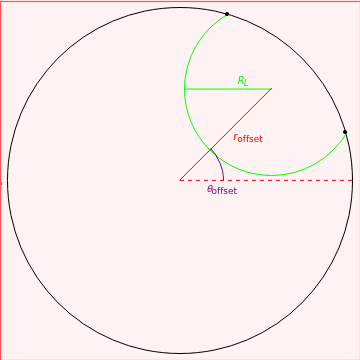
\includegraphics{img/continuous_pair_corrections}
			\caption{The continuous and discretized calorimeters for phase space and discretization efficiency correction to smooth distribution and reduce bin width selection dependence}
		\end{center}
		\label{fig:eff_corr}
	\end{figure}
	Thus, the full efficiency correction on $\Delta R_L$ to correct for both edge effects of the jet cone and the effects of a finite spatial resolution on the calorimeters is 
	\begin{equation}
		\begin{split}
			\varepsilon \left( R_L, R_j, \delta \right) &= \frac{R_L r_2 \left( \frac{R_L^2}{\delta^2} \right)}{2 \pi R_j^2 } \left[  \frac{\sqrt{4 R_j^2 -R_L^2} + R_j E \left( \textrm{arccos} \left( \frac{R_L}{2R_J} \right) \left| \frac{R_L^2}{R_j^2} \right. \right) } {r_2 \left( \frac{R_L^2}{\delta^2} \right) -  \left. \sum^{\frac{\left(R_j + R_L \right)^2}{\delta^2}i}_{i=\frac{R_j^2}{\delta^2}} r_2(i) \right/ \sum^{\frac{R_j^2}{\delta^2}i}_{i=0} r_2(i) }  \right]
		\end{split}
	\end{equation}
\section{Uncertainties}
	\subsection{Statistical Uncertianity}

	\subsection{Systematic Uncertianity sources}
	\subsection{Binning Uncertianity}
	\subsection{Systematic Uncertainties}

\part{Technicalities: The finer points of theory and computing}
\chapter{The Energy Correlator and the primary vertex}
	\label{ch:ENC_th}
	Considering the limitations of Calorimetry only measurement with RHIC one is 
So the energy correlator allows a look back, I guess that's the relevant bit? 
	Point being, if the jet points back to the primary vertex, the share of the energy between the jets and the composition of those jets is directly determined by the $2 \rightarrow 2$ scattering and is thus sensitive to the parton distribution functions of the beam particles. 
	Starting from the definition of the energy correlator given in \cite{Larkoski2013}:
	\begin{equation}
		\mathcal{E}_{N} = \int \frac{\dd \Omega}{2} \int \dd \vec{n}_{12} \frac{\langle \varepsilon \left( \vec{n}_1 \right) ... \varepsilon \left(\vec{n}_2 \right)\rangle}{Q^2} \delta\left( \vec{n}_1 \cdot \vec{n}_2 - 2|\vec{n}_1|||\vec{n}_2|\cos  \theta \right)
		\label{eq:ENC}
	\end{equation}
	Where $\varepsilon \left( \vec{n}_i \right)$ is the energy flow operator defined as 
	\begin{equation}
		\varepsilon \left( \vec{n}_i \right) = \lim_{r\rightarrow \infty} r^2 \int_{-\infty}^\infty \dd t \vec{n}^i T^0_{i}\left( t, r \vec{n} \right) 
		\label{eq:enrgy_flow_op}
	\end{equation}
	\section{The primary vertex and interaction}
	The goal of this work is to extract gluon distributions from the jet, thus one must consider those initial verticies that (to first order) produce the gluon-quark, gluon-gluon, and quark-quark dijet events. 
	To this end, one considers the following tree level diagrams 
	\begin{figure}
		\begin{centering}
			\begin{tikzpicture}[scale=0.7]
				\begin{feynman}
					\vertex(a);
					\vertex[below=3cm of a](b);
					\vertex[below=1.5 cm of a](c);
					\vertex[right=2 cm of c](d);
					\vertex[right=2 cm of d](e);
					\vertex[right=6 cm of a](f);
					\vertex[right=6 cm of b](g);
					\diagram*{
						(a)--[gluon](d);
						(b)--[gluon](d);
						(d)--[gluon](e);
						(e)--[fermion](f);
						(g)--[fermion](e);
					};
				\end{feynman}
			\end{tikzpicture}
			\begin{tikzpicture}[scale=0.7]
				\begin{feynman}
					\vertex(a);
					\vertex[below=3cm of a](b);
					\vertex[below=1.5 cm of a](c);
					\vertex[right=2 cm of c](d);
					\vertex[right=2 cm of d](e);
					\vertex[right=6 cm of a](f);
					\vertex[right=6 cm of b](g);
					\diagram*{
						(a)--[fermion](d);
						(d)--[fermion](b);
						(d)--[gluon](e);
						(e)--[fermion](f);
						(g)--[fermion](e);
					};
				\end{feynman}
			\end{tikzpicture}
			\caption{ $p+p\rightarrow q \bar{q} + X$ events, these dijet-types are possible to be produced from gluon or quark interchange, probing the square of the gluon or quark distributions}
			\label{fig:qq_jets_fd}
		\end{centering}
	\end{figure}
	\begin{figure}
		\begin{centering}
			\begin{tikzpicture}[scale=0.7]
				\begin{feynman}
					\vertex(a);
					\vertex[below=3cm of a](b);
					\vertex[below=1.5 cm of a](c);
					\vertex[right=2 cm of c](d);
					\vertex[right=2 cm of d](e);
					\vertex[right=6 cm of a](f);
					\vertex[right=6 cm of b](g);
					\diagram*{
						(a)--[gluon](d);
						(b)--[gluon](d);
						(d)--[gluon](e);
						(e)--[gluon](f);
						(g)--[gluon](e);
					};
				\end{feynman}
			\end{tikzpicture}
			\begin{tikzpicture}[scale=0.7]
				\begin{feynman}
					\vertex(a);
					\vertex[below=3cm of a](b);
					\vertex[below=1.5 cm of a](c);
					\vertex[right=2 cm of c](d);
					\vertex[right=2 cm of d](e);
					\vertex[right=6 cm of a](f);
					\vertex[right=6 cm of b](g);
					\diagram*{
						(a)--[fermion](d);
						(d)--[fermion](b);
						(d)--[gluon](e);
						(e)--[gluon](f);
						(g)--[gluon](e);
					};
				\end{feynman}
			\end{tikzpicture}
			\caption{ $p+p\rightarrow gg + X$ events, these dijet-types are possible to be produced from gluon or quark interchange, probing the square of the gluon or quark distributions}
			\label{fig:gg_jets_fd}
		\end{centering}
	\end{figure}
	\begin{figure}
		\begin{centering}
			\begin{tikzpicture}
				\begin{feynman}
					\vertex(a);
					\vertex[below=3cm of a](b);
					\vertex[below=1.5 cm of a](c);
					\vertex[right=2 cm of c](d);
					\vertex[right=2 cm of d](e);
					\vertex[right=6 cm of a](f);
					\vertex[right=6 cm of b](g);
					\diagram*{
						(a)--[fermion](d);
						(d)--[gluon](b);
						(d)--[fermion](e);
						(e)--[gluon](f);
						(e)--[fermion](g);
					};
				\end{feynman}
			\end{tikzpicture}
			\caption{ $p+p\rightarrow gq \left(\bar{q} \right) + X$ events, these dijet-types are possible at the tree level only via quark (antiquark) and gluon interactions, hence probing both gluon and quark distributions at once}
			\label{fig:qg_jets_fd}
		\end{centering}
	\end{figure}
	% gotta actually make these Feynman diagrams
	While the processes are not imediately apparent in the final state of the jet, one notes that the two and three point energy correlators give a useful distinction as the jet function can be divided out, leaving a vertex dependent term at $R_L \approx 2 R_{\textrm{jet}}$
	%vertex dependent terms from OPE of the energy flow 
\chapter{Jets in Vacuum and the PDF}
\section{Jet Identification Algorithms}
\label{sec:toy_jet_id}
As discussed in chapter \ref{ch:LR}, there are a variety of jet finding algorithms that prioritize different theoretical aspects of the underlying physics while being experimentally realizable \cite{Dokshitzer1997} \cite{Atkin2015}. 

In general, a jet identification algorithm needs to be IRC safe. 
That is, the jet object needs to display invariance in the Infrared (IR) and Collinear regimes, managing real-virtual cancellation and keeping results meaningful for emission and splitting respectively. 

\chapter{So exactly how intelligent is AI}

%\chapter{Proof Solving and Validation as Quality Control Mechanisms}

